%% Website of the LaTeX Gods: https://en.wikibooks.org/wiki/LaTeX
\documentclass[11pt, titlepage]{article}
%%%%%%%%%%%%%%%%%%%%%%%%%%%%%%
% STARTING DOCUMENT PREAMBLE %
%%%%%%%%%%%%%%%%%%%%%%%%%%%%%%

\usepackage[utf8]{inputenc}
\usepackage[a4paper, margin=2cm]{geometry}
%taken from sysReq:
\linespread{1.2}
\setlength{\parindent}{0pt}
\setlength{\parskip}{1em}
%

% Taken from acceptanceCriteria
\usepackage{tabu}
\usepackage[table, usenames, dvipsnames]{xcolor}
\usepackage{booktabs,colortbl,longtable}
\usepackage{graphicx}
\usepackage{lscape}
\usepackage[strict]{changepage}
%

% Taken from agileSoftwareDevelopment
\usepackage{pdfpages}
\usepackage[english]{babel}
%\usepackage[backend=bibtex,bibencoding=ascii]{biblatex}
\usepackage[style=authoryear,backend=bibtex,bibencoding=ascii]{biblatex}
\usepackage{csquotes}
\addbibresource{./bibliographies/agileSoftwareDevelopment}
\addbibresource{./bibliographies/lsepi.bib}
\usepackage{enumerate}
\usepackage[titletoc]{appendix}
%

\usepackage{pdflscape}

\usepackage{anyfontsize}
\usepackage{titlesec}
\usepackage{url}
\usepackage[shortlabels]{enumitem}

\title{First Report}
\author{Group 9}

\newcommand{\makeColourful}{\color{MidnightBlue}}
\newcommand{\makeGrey}{\color{Gray}}
\newcommand{\makeBlack}{\color{Black}}
\renewcommand*\contentsname{\fontsize{25}{30}\selectfont Table of Contents}
\renewcommand{\thesection}{\Roman{section}}

\titleformat{\section}{\LARGE \bfseries \makeColourful}{\thesection}{0.7cm}{}[{\hrule}]
\titleformat{\subsection}{\Large \bfseries \makeColourful}{}{0}{}[]
\titleformat{\subsubsection}{\large \bfseries \makeColourful}{}{0}{}[]
\titleformat{\subsubsubsection}{\normalsize \bfseries \makeColourful}{}{0}{}[]
\titleformat{\subsubsubsubsection}{\normalsize \bfseries \makeColourful}{}{0}{}[]

%%%%%%%%%%%%%%%%%%%%%%%%%%%%
% ENDING DOCUMENT PREAMBLE %
%%%%%%%%%%%%%%%%%%%%%%%%%%%%
\begin{document}
	\begin{titlepage}
		\newcommand{\HRule}{\rule{\linewidth}{1.5mm}}
		\center
		\begin{minipage}{0.4\textwidth}
			\begin{flushleft}
				\textbf{\large CM2305}
				\\
				\emph{\large Group Project}
			\end{flushleft}
		\end{minipage}
		~
		\begin{minipage}{0.4\textwidth}
			\begin{flushright}
				\textbf{\large Module Leader}
				\\
				\emph{\large Frank \textsc{Langbein}} 
			\end{flushright}
		\end{minipage}
		\\[2cm]
        
		{\makeColourful \HRule} 
		\\[2cm]
		{\fontsize{90pt}{0pt}\selectfont \makeColourful{\textsc{First Report}}}
		\\[1.5cm]
		A \LaTeX\ document
		{\makeColourful \HRule}
		\\[3cm]
        ~
		\begin{minipage}{0.4\textwidth}
			\begin{flushright} \large
				\emph{Clients:} \\
				\mbox{Stuart \textsc{Allen}}, \mbox{Dafydd \textsc{Evans}}
			\end{flushright}
		\end{minipage}\\[3cm]
		\textsc{\Large Group 9}
		\\[0.5cm] 
		\textsc{Aimi Daros, Braden Marshall, Cameron Fish, Lucy Robertshaw, Mariza Celliers, Ryan Flynn, Sh’kyra Jordon, Skye Watkins, Thomas Rice.}
	\end{titlepage}
	\newpage
	\tableofcontents
	\newpage
	\subsection{Revised Requirements}
	For the development of CAMEL we have decided to revise some of the existing requirements that we proposed in the first report. We have decided to change a few of the requirements as we have decided to go with a different approach to development than we originally intended in the first report.\\
	
	\textbf{New Requirements}
	\begin{itemize}
		\item New parser implementation
		\item Re-factoring of existing codebase
	\end{itemize}
	
	\documentclass[12pt]{article}

\usepackage{geometry}
\geometry{a4paper}

\usepackage{url}

\linespread{1.2}

\setlength{\parindent}{0pt}
\setlength{\parskip}{1em}

\begin{document}
	\begin{titlepage}
		\newcommand{\HRule}{\rule{\linewidth}{0.5mm}}

		\center

		\textsc{\LARGE Cardiff University}\\[1.5cm]
		\textsc{\Large Computer Science}\\[0.5cm]
		\textsc{\large CM2305: System's Design \& Group Project}\\[0.5cm]

		\HRule \\[0.4cm]
		\textsc{\Large \textbf{CAMEL}}\\[0.1cm]
		\textsc{\Large \textbf{CA}rdiff \textbf{M}athematics \textbf{E-L}earning}\\[0.7cm]
		{\huge\bfseries Requirements}\\[0.4cm]
		\HRule \\[1.5cm]

		\begin{minipage}{0.4\textwidth}
			\begin{flushleft} \large
				\emph{Authors:}\\
				\mbox{Mariza \textsc{Celliers}}, \mbox{Ryan \textsc{Flynn}}, \mbox{Braden \textsc{Marshall}}
			\end{flushleft}
		\end{minipage}
		~
		\begin{minipage}{0.4\textwidth}
			\begin{flushright} \large
				\emph{Clients:} \\
				\mbox{Stuart \textsc{Allen}}, \mbox{Dafydd \textsc{Evans}}
			\end{flushright}
		\end{minipage}\\[3cm]

		{\large \today}\\[2cm]

		\vfill
	\end{titlepage}


	\tableofcontents

	\newpage
	\section{System Scope}
	The proposed project that has been put forward to us, is to update and complete the implementation of the current CAMEL system. The existing codebase needs additional functionality, which includes lexical comparisons, logging of student answers and deadline functionality . On top of providing a improved system, documentation and unit tests will also be included.

	To address the clients proposal, CAMEL 2.0 will issues a code standard. This will be PEP8 Python standard, and will be the first priority to implement to the system. Additionally, exception handling will also be added as well as extra code to fix any current bugs that reside. Besides maintaining the code, documentation for a developer and administrator will be added. All of this will be part of an ongoing process during development, with each being equally important.   
	
	Addressed functionality (see  functional requirements) will be implemented in agile sprints, the length of the sprint cycle for functionality is dependant on the complexity. For example, lexical comparisons may take longer than adding exception handling, due to the complexity that is required to add this into the codebase. Other functionality, such as database re-design and break down of core functionality will be allotted a time frame during the sprint cycle meetings. The plans for the cycles will be drawn up every week during the implementation stage.   
	
	Tests will be added prior to writing the code, though will be written in Django's test framework first. Additional or 'conceptual' functionality will be addressed last, to ensure high code quality throughout. However, due to a fixed time frame, we will only be implementing functionality that is mentioned in the requirements. No additional requirements later on will be added.          	
	\section{Assumptions}
	Due to the fixed nature of the current system, there are some aspects that we will need to assume. Firstly, we are assuming that the functionality we are developing for is single threaded. This assumption is being made as the time scale to add threaded functionality is non-existent. Furthermore, we are developing the system on Django's development server, which cannot simulate a multi-threaded environment. 
	
	A further assumption we are making is that there will be no additional requirements added when implementation occurs, and these requirements are final. Given the time scale we have to make the system, it would be unlikely that any additional requirements could be completed to a high standard. Any additional functionality will be dropped due to development scope. 
	
	Finally, we area assuming that the use of third party software to handle aspects that are out of scope can be integrated into the system. Third party applications that may be include:
	\begin{itemize}
		\item JQuery - JavaScript Library
		\item Bootstrap - CSS Library
		\item Additional Python modules
	\end{itemize}
	\section{Functional Requirements}
	\subsection{Add methods of checking and comparing student answers from questions. - R}
	To meet the initial requirement of lexical analysis, functionality will need to be added to current student answers to be compared. Functionality that can be included may be graphs and statistics. With this functionality, lecturers are able to see possible trends with particular pieces of work, and see if there are any issues. This functionality can also be expanded as a plagiarism checker, by looking for common answers. The depth of functionality that could be provided is limited to the development scope.
	\subsection{Logging of Student Answers}
	As the primary goal of the system is to allow members of staff to upload tests - in the form of LaTeX documents - with 'interactive' answering features, for the students to access, answer and submit; it seems only natural that these submissions are to be logged and then viewable by the supervising members of staff. A time-stamp should be attached to each submitted answer to allow a deeper understanding of student upload patterns.
	\subsection{Add deadlines to student homework questions which will prevent late submissions. - M}
	In the brief it specifies that there should be capabilities to ‘complete and submit homework assignments’ and our client has also outlined that a way of adding deadlines to homework questions is something that should be implemented on the system.
By being able to have deadlines on homework submissions, it would ensure the solutions of the students who miss the deadlines are not marked and their score is not added to their overall grade. It would also allow the grades of these students to not be included in the analysis and comparison of the classes grades.
After a deadline has passed for a specific coursework, the student should be able to see and write answers for the questions, but not be able to submit it.  And the lecturer should be able to see which students have not submitted.
A lecturer should also have the option of choosing not to set a deadline.

	\subsection{Provide functionality to only see modules a student is enrolled for. - R}
	This requirement will be a proof of concept rather than a fully functional feature, due to not having the permissions to access enrolment data. The concept will instead simulate some test data to assess the possibility of this feature being added. If the concept is a success, it will allow the UI for the student to be simple, as it will only show their enrolled modules. This adds to ease of use, however this feature is not detrimental to the final system. The functionality of these feature is dependent with time available.
	\subsection{Input Error Checking}
	In the current version of the system, when the contents of a LaTeX document is passed into the LaTeX parser, there is virtually no validation of this input. The input is wrongly assumed to be already correctly formatted. Although our client informed us that adding validation functionality for the staff uploaded LaTeX test documents was not a necessity, he did request that any arising errors should be safely dealt with i.e. not cause a system crash or corrupt the database.
	\subsection{Provide exception handling. - M}
	In the brief is specifically states that the existing codebase has no exception handling, and that this needs to be added. By speaking to our client this is a requirement that is of a high priority and will have to be implemented.
The exception handling in the system would enable us to find and fix bugs easily and quickly during production, it would also enable the code to be maintainable in the future and it would also allow for smooth running for the system.

	\subsection{Provide Unit Tests. - R}
	All code that is developed will utilise the Django’s already existing test framework, along with Python’s testing mechanics. This will be a continuous process in the development sprints. Though all tests will be created first, before code is written. This will give a good indication of the time each feature requires to be implemented. By having the tests drawn up first, we allow the requirement to be flexible, and have the ability to make changes if issues occur. It also allows possible extensions to be added in the future, as test first development ensures high code quality. This will also meet the requirement proposed in the brief by including these tests. These tests can be utilised by future developers using Django.

	\newpage
	
	\section{Non-Functional Requirements}
	\subsection{Fix Bugs in the Current System}
	The current system, as it stands, is in no way acceptable for deployment. There exists an unknown amount of bugs and several poor design-choices which desperately require fixing for the project to be a success. If these issues are not dealt with accordingly, their impact will greatly hinder development and the system would be left unreliable and potentially dangerous.
	\subsection{Improve navigation reliability when moving between pages - B}
	When navigating around the current system, it seems that many of the hyper-links are incorrectly using relative address references - as oppose to absolute or referring to the root domain. This results in users of the system being miss-directed when navigating around the site. It even makes some areas of the site completely unacceptable without the user manually changing the file path.  This is likely due to the incorrect usage of Django's URL template tag\footnote{\url{https://docs.djangoproject.com/en/stable/ref/templates/builtins/#url}} and should be solvable without a huge amount of issues.
	\subsection{Ease of use - M}
	In the brief it states that ‘the way in which students and teachers interact with the system should also be investigated and the design modified accordingly’. Our client has also made it clear that they would like the system easy enough for the students and teachers to use so that they will not need documentation, and should be intuitive and straight forward to navigate and find the needed information easily.
	\subsection{Administrator and Developer documentation. - R}
	Documentation will be required to meet a proposed requirement. The main focus for the documentation will be for the developer, which will focus on the technical aspects. It will include details on functionality on particular files and certain standards in the code. The administrator documentation will be 'lightweight' and will include all the instructions and commands that are needed to operate the system. Though the developer documentation will be considered a higher priority over the administrator, due to the UI being self explanatory. The documentation will be accessed on the site itself for both developer and administrator. 
	\subsection{System Permissions}
	The system currently features two different types of users - students and staff members. It is required that various additional permission parameters are to be attached to the staff accounts, so that only they are able to access the sensitive areas of the system. These sensitive areas include:
	\begin{itemize}  
        \item LaTeX test document upload point
        \item LaTeX test document manage point
        \item List of the registered students
        \item List of the student's test results
    \end{itemize}
    Depending on time restraints, it is advisable that Django's automatic admin interface\footnote{\url{https://docs.djangoproject.com/en/stable/ref/contrib/admin/}} not be accessible by staff members. This is because it is an extremely powerful tool that could easily be misused and permanently damage the system's stored data.

	\subsection{Upgrade System for Python3. - M}
	After discussing with our client, upgrading to Python 3 is an optional requirement depending on how easy this change would be and how long that it would take us to change the existing codebase. 
We would want to move to python 3 as majority of the IO issues have been worked out, and python 2 will eventually become obsolete. By changing to python 3 it means that the system will be more maintainable as more people will know this release of python, and the system would be compatible with more devices for a longer period of time.

	\subsection{Have maintainable code. - R}
	Throughout the development cycle, the aim will be to update and add code that follows a set of standards. These standards will include comments, naming conventions and modularity of files. For this project, we have been instructed to use the PEP8 Python standard. This standard focuses on using underscores for naming conventions. Upon bringing these standards, it will ensure that future developers will be able to quickly understand the context of a code and continue to maintain high the system for the future.
	
	\subsection{Modify database to allow tables for Student, Teacher, Author, Admin. - M}
	Our client has also mentioned to add four more tables into the database to be able to be able to ensure no data is lost and kept in an organised manner for if it needs to be manually accessed. It would also ensure that these attributes can be easily referenced and compared throughout the system.
	
	\subsection{Break down the core code to become smaller 'applications' in Django. - M}
	After the third meeting with our client, he has specified specifically that he would like the code to be broken down and organised into the correct Django ‘applications’. By doing this the Code will be better organised and easier to understand by others therefore more maintainable. If the code was better split up into the applications, it would also cause code reuse to be easier throughout the application, later on if the system expands, or is released to be downloaded and used by the public.
\end{document}

	\documentclass[12pt]{article}

\usepackage[utf8]{inputenc}
\usepackage[a4paper, margin=1in]{geometry}

\usepackage{xcolor}
\usepackage{booktabs,colortbl,longtable}

\linespread{1.2}

\setlength{\parindent}{0pt}
\setlength{\parskip}{1em}

\begin{document}
	\begin{titlepage}
		\newcommand{\HRule}{\rule{\linewidth}{0.5mm}}

		\center

		\textsc{\LARGE Cardiff University}\\[1.5cm]
		\textsc{\Large Computer Science}\\[0.5cm]
		\textsc{\large CM2305: System's Design \& Group Project}\\[0.5cm]

		\HRule \\[0.4cm]
		\textsc{\Large \textbf{CAMEL}}\\[0.1cm]
		\textsc{\Large \textbf{CA}rdiff \textbf{M}athematics \textbf{E-L}earning}\\[0.7cm]
		{\huge\bfseries Acceptance Criteria}\\[0.4cm]
		\HRule \\[1.5cm]

		\begin{minipage}{0.4\textwidth}
			\begin{flushleft} \large
				\emph{Authors:}\\
				\mbox{Lucy \textsc{Robertshaw}}, \mbox{Cameron \textsc{Fish}}, \mbox{Skye \textsc{Watkins}}
			\end{flushleft}
		\end{minipage}
		~
		\begin{minipage}{0.4\textwidth}
			\begin{flushright} \large
				\emph{Clients:} \\
				\mbox{Stuart \textsc{Allen}}, \mbox{Dafydd \textsc{Evans}}
			\end{flushright}
		\end{minipage}\\[3cm]

		{\large \today}\\[2cm]

		\vfill
	\end{titlepage}


	\tableofcontents

	\newpage
	
	\section{Testable acceptance criteria}
	\begin{itemize}
	\item The lecturer can set a deadline to a piece of homework after which time, the system will not accept submissions.
	\item The system will make a log of all homework submissions.
	\item The system can compare different homework logs for similarity.
	\item The system can auto mark simple ‘tick-a-box’ style questions.
	\item The system will only allow a student to see content for the module they are enrolled on.
	\item If someone tries to submit Latex that contains errors, the system will stop them.
	\item All errors are handled without system failure.
	\item Unit testing has been completed.
	\item The system has no known bugs.
	\item The end user requires no instruction or documentation on how to navigate the system as it is both simple and easy to use.
	\item Documentation has been completed for system Admins and Developers.
	Students cannot access lecturer-only areas.
	\item The code is written in Python3.
	\item The code is easily readable for maintenance and development.
	\end{itemize}
	

    \newpage
    
	\section{Risks and Benefits}
		\subsection{Risk Assessment}
			\definecolor{greenI}{RGB}{226, 239, 217}
			\definecolor{greenII}{RGB}{197, 224, 179}
			\definecolor{greenIII}{RGB}{0, 176, 80}
			
			\definecolor{yellowI}{RGB}{255, 229, 153}
			\definecolor{yellowII}{RGB}{255, 255, 0}
			
			\definecolor{orangeI}{RGB}{244, 176, 131}
			\definecolor{orangeII}{RGB}{255, 165, 0}
			
			\definecolor{redI}{RGB}{255, 150, 150}
			\definecolor{redII}{RGB}{255, 0, 0}
			
			\subsubsection{Key}
				\begin{table}[!htb]
					\begin{center}
						\caption{Risk Assessment Key}
						\label{table:riskassessmentkey}
						\setlength{\aboverulesep}{0pt}
						\setlength{\belowrulesep}{0pt}
						\setlength{\extrarowheight}{.75ex}
						\begin{tabular}{|*{6}{p{2cm}|}}
							\toprule
							Total Risk & \multicolumn{5}{c|}{Impact} \\
							\midrule
							
							Likelihood of Happening & \cellcolor{greenI}1.Insignificant {\scriptsize (Minor problem easily handled)} & \cellcolor{greenII}2.Minor {\scriptsize (Some disruption possible)} & \cellcolor{yellowI}3.Moderate {\scriptsize (Significant time/resources required)} & \cellcolor{orangeI}4.Major {\scriptsize (Project severely damaged)} & \cellcolor{redI}5.Catastrophic {\scriptsize (Project ruined)}\\
							\midrule
							
							\cellcolor{greenI}1.Highly Unlikely & \cellcolor{greenIII}1 Low & \cellcolor{greenIII}2 Low & \cellcolor{greenIII}3 Low & \cellcolor{yellowII}4 Moderate & \cellcolor{yellowII}5 Moderate\\
							\midrule
							
							\cellcolor{greenII} 2.Unlikely & \cellcolor{greenIII}2 Low & \cellcolor{yellowII}4 Low & \cellcolor{yellowII}6 Moderate & \cellcolor{orangeII} 8 High & \cellcolor{orangeII}10 High\\
							\midrule
							
							\cellcolor{yellowI}3.Moderate & \cellcolor{greenIII}3 Low & \cellcolor{yellowII}6 Moderate & \cellcolor{orangeII}9 High & \cellcolor{redII}12 Extreme & \cellcolor{redII}15 Extreme\\
							\midrule
							
							\cellcolor{orangeI}4.Likely & \cellcolor{yellowII}4 Moderate & \cellcolor{orangeII}8 High & \cellcolor{redII}12 Extreme & \cellcolor{redII}16 Extreme & \cellcolor{redII}20 Extreme\\
							\midrule
							
							\cellcolor{redI}5.Almost Certain & \cellcolor{yellowII}5 Moderate & \cellcolor{orangeII}10 High & \cellcolor{redII}15 Extreme & \cellcolor{redII}20 Extreme & \cellcolor{redII}25 Extreme\\
							\bottomrule
						\end{tabular}
					\end{center}
				\end{table}
			    	
				In order to assess the risks of our project we included the use of a risk map. Firstly we identified the risk that could occur in the duration of our project and then described the effect it would have upon the group. We calculated the total risk by measuring the likelihood of the event occurring, against the impact it would have should it occur. The controls include the contingency, avoidance and how we would cope with the risk if it occurred. This helps us to maintain the project goals and control the overall risk. After the controls are implemented, we then measured the total risk again in the hope it would have improved. We followed the colour schemes of the risk map so it is more visually appealing and clearer to assess how the controls we implemented help. We aimed to achieve the colours of green and yellow for the total risk given the controls. We then analysed the benefits of having the risk controls in place for each risk, and explained the benefits as a paragraph as many interlinked.
		     
		    \subsubsection{Risk Assessment Table}
				\label{table:riskassessment}
				\setlength{\aboverulesep}{0pt}
				\setlength{\belowrulesep}{0pt}
				\setlength{\extrarowheight}{.75ex}
				\begin{longtable}{|*{5}{p{2.5cm}|}}
					\caption{Risk Assessment} \\
					\toprule
					Risk & Effect & Total Risk \scriptsize (Likelihood * Impact) & Controls & Total Risk Given Control \scriptsize (Likelihood * Impact) \\
					\midrule
					\endfirsthead
					\multicolumn{5}{c}%
					{\tablename\ \thetable\ -- \textit{Continued from previous page}} \\
					\midrule
					Risk & Effect & Total Risk \scriptsize (Likelihood * Impact) & Controls & Total Risk Given Control \scriptsize (Likelihood * Impact) \\
					\midrule
					\endhead
					\hline \multicolumn{5}{r}{\textit{Continued on next page}} \\
					\endfoot
					\midrule
					\endlastfoot
					
					Short-term Illness of team member & Parts of the project may not be complete and the whole team might miss a crucial deadline in regards to when the work is due in. A delay in the project could be caused.  & \cellcolor{yellowII} 6 (3 * 2) & Regular de-briefing with group so all know what each member has done and will do.
					Write comments on major updates onto GitHub when committing.
					If it does happen, tasks for that member will be fairly re-assigned to other members. & \cellcolor{greenIII}3 (3 * 1)\\
					\midrule
					
					Team member leaving the group & The effect on the team will be major. Potential delays with areas of the specification/code, or possibly no access to the documentation. & \cellcolor{yellowII} 5 (1 * 5 ) & Regular de-briefing with group so all know what each member has done and will do.
					
					If it does happen, tasks for that member will be fairly re-assigned to other members. & \cellcolor{yellowII} 4 (1 * 4)\\
					\midrule
					
					Loss of work (eg. due to corrupt files or forgetting to save) & The effect of this would be major if the loss was of lots of work and was nearing close to handing in date. & \cellcolor{orangeII} 9 (3 * 3) & Use of GitHub/Google Drive/auto-saving software.
					Everyone will save their work at least every 20 minutes.
					Routine backups will be made every week.
					Create a Gantt chart specifying every task to be completed and follow it. 
					
					If it does happen we will find the latest version of the work and schedule in the nearest available time to re-do the missing work. & \cellcolor{yellowII} 4 (2 * 2) \\
					\midrule
					
					Overrun on a task and miss a milestone & Delay on work, could cause a knock-on effect of hold ups and delays, thus risking not reaching milestones, and possibly not completing the project on time. & \cellcolor{redII} 12 (3 * 4) & Thorough planning of each task and appropriate deadlines with regular de-briefing with group so all know what is on schedule. 
					Create a gantt chart specifying every task to be completed and follow it. 
					
					If it does happen we will schedule in the nearest available time to complete the given task, and more group members can help the individual or sub team who have overrun. & \cellcolor{yellowII} 6 (2 * 3) \\
					\midrule
					
					Not all functional requirements are met by the deadline. & Parts of the project may not be complete and the whole team might miss a crucial deadline in regards to when the work is due in. A delay in the project could be caused. & \cellcolor{redII} & Agree reasonable functional requirements with client. 
					Plan time well.
					Use of agile model could allow for adjustments of requirements.
					
					\textbf{If it does happen nothing can be done!} & \cellcolor{yellowII} 5 (1 * 5) \\
					\midrule
					
					Client indisposed & Client criteria might not be met, potential hold ups to project progression. & \cellcolor{yellowII} 6 (3 * 2) & Fully understand task and fully document requirements as and when they’re agreed.
					
					If it does happen we should ensure we are regularly having meetings with the client and try to resolve any issues we may have as soon as possible. & \cellcolor{greenIII} 3 (3 * 1) \\
					\midrule
					
					Team member prolonged absence & The effect on the team will be major. Potential delays with areas of the specification/code, or possibly no access to the documentation. & \cellcolor{greenIII}  3 (1 * 3) & Regular de-briefing with group so all know what each member has done and will do.
					
					If it does happen, tasks for that member will be fairly re-assigned to other members. & \cellcolor{greenIII} 2 (1 * 2) \\
					\midrule
					
					Server failure (e.g., GitHub goes down, files incompatible with server) & The effect of this would be major if the loss was of lots of work and was nearing close to handing in date, or work was inaccessible during presentation. & \cellcolor{yellowII} 4 (1 * 4) & Routine backups will be made every week on hardware (eg USB)  and other alternative software.
					
					If it does happen we will find the latest version of the code that is backed up on another device, either from hardware or software and fill in any gaps that are missing at the earliest convenience. & \cellcolor{greenIII} 3 (1 * 2)\\
					\midrule
					
					Django gets updated & Parts of the code would be unusable and cause bugs, and as a result may need updating/changing. This would take time. & \cellcolor{greenIII} 3 (1 * 3) & Make sure code is well-structured and documented.
					
					
					If it does happen we will use the latest version of the work and schedule in the nearest available time to re-do the missing work. & \cellcolor{greenIII} 2 (1 * 2) \\
					\midrule
					
					Code corrupted, unusable or deleted & This would be a medium effect on the team, as work may need to be remade. & \cellcolor{redII} 12 (3 * 4) & Use of GitHub/Google Drive/auto-saving software.
					Everyone will save their work at least every 20 minutes.
					Routine backups will be made every week.
					
					If it does happen we will find the latest version of the work and continue from there again. & \cellcolor{yellowII} 4 (1 * 4) \\
					\midrule
					
					Last minute bugs, 1 hour before deadline & The consequences would be major in the event of failure to show the completed project and possibly the loss of marks.  & \cellcolor{redII} 15 (3 * 5) & Have multiple people do thorough debugging on different systems.
					
					If it does happen we will ensure two group members check over the code for any final bugs before submission. If any are found they should be fairly easy to resolve as  our code will be organised. & \cellcolor{yellowII} 5 (1 * 5)\\
					\bottomrule
				\end{longtable}
				
			\newpage
			
			\subsubsection{Controls}
				\begin{itemize}
					\item Use of google drive
					\item Use of github
					\item Write comments on major updates onto github when committing.
					\item Use of auto-saving software
					\item Save work at least every 20 minutes.
					\item Use of agile model.
					\item Meeting weekly to de-brief.
					\item Regularly updated time-plan.
					\item Agree reasonable functional requirements
					\item Fully document requirements
					\item Routine backups of work made every week.
					\item Thorough planning of each task for time management.
					\item Make sure code is well-structured and documented.
					\item Have multiple people do thorough debugging on different systems.
					\item Create a gantt chart specifying every task to be completed and follow it. 
				\end{itemize}

		\subsection{Benefits}

			By conducting our risk assessment we are able to prepare backup plans by writing out all potential risks, and creating controls to minimise the impacts they may have on our group project. We can easily recognise and control risks in the project the clear structure presented. Our Risk Assessment can be used as a referral tool for all members of the group. It creates awareness to the group members, the group is able to undergo controls to reduce the possible risks. With our contingency plan in place, we are also able to save time and effort if in the unlikely event of the risk occurring, thus causing minimal amount of damage to our project as possible. 

		\newpage
    
	\section{Relevant Quality Factors}
		\textbf{Flexibility and Extensibility}  

		Our software will be very flexible should the client need to modify, remove or add any functionality at a later date. Any requirements that are changed by the client will be easily found within the code, as we are going to document the code so it is clear which part relates to which section of the Camel website or database. Through documentation we can quickly access the required code and fulfil the clients specification change without affecting our system as a whole. This allows extensibility as the system will not be damaged through adding or modifying functionality. As our clients could change their minds on the requirements at any time this is a crucial and relevant quality factor we need for our software. 

	    \textbf{Maintainability and Readability}   
    
		Similar to the flexibility aspects of our project, the code will be maintainable should it need to be modified for any corrections. If a bug was to be found at a later date it would be easy to find the section it is related to. The code will be readable through documentation so we can see what the code is trying to do, and try to fix it accordingly. The readability of our code is being maintained through each user documenting their code before uploading it to the GitHub file share. The more documentation we include, the more maintainability can be achieved.

		\textbf{Performance and Efficiency} 
    
		Our software should react with a quick response time and not have any time delays when the students or lecturers are uploading work. The performance of the response time should only take a few seconds to ensure it is friendly to the user. Efficiency of our software can be increased with resource utilisation and we can ensure performance is achieved by measuring the time it takes to upload an homework assignment. 

		\newpage
    
	    \textbf{Scalability}   
    
		In relation to performance, the scalability quality factor is also relevant to the software we are fixing and redeveloping. The software system should respond to any actions taken by the user in an acceptable duration of time, independent of what the load size is. The hardware in which the software is being used all also affects scalability so we should ensure the software works within the Windows and Linux labs. Our system will have scalability, meaning the ability of being able to run the interactive website on an increasing amount of machines, handling increasing user interaction, as this will be required for in class tests within the lab environment. We can test the scalability of our software to ensure it is performing to standard by checking its ability to accommodate rising resource demand. All members who want to access Camel should be able to whenever they want, independent of the amount of students logged in. We could calculate the throughput and the resource usage to discover the system's scalability.
        
		\textbf{Availability, Fault Tolerance and Reliability}   

		Our software will integrate the quality factors of availability, fault tolerance and reliability. It should always be available for the user to access the information within it online for a high percentage of the time. It should also still continue to run even if parts are being added or modified. Reliability can be maintained through ensuring the code we create is copied to multiple devices and it is enhanced by features that helps to avoid,detect and repair any faults. We are undertaking a paired programming approach when we implement our code so the software can be more reliably monitored for any changes, and include improved fault tolerance. If it was to crash when deployed, it could be recovered from backed up sources with fault tolerance approaches.

		\newpage
	
	    \textbf{Usability and Accessibility}   

		Our project has an existing user interface. It is basic in appearance, and will most likely be overhauled upon completion, and rebranded with the university colours. As the project is focused on the functional task of making it work, we will not need to create a user interface. The current user interface is clear in colours and suits our prototype. It is simple and provides wide accessibility for the user. Its navigation is clear and obvious, making the website easily traversable. We will continue to uphold this standard throughout the project, and any parts that we add will be intuitive without any need for documentation. 

		\textbf{Platform Compatibility and Portability  }     

		As our project is browser based, we do not need to be aware of functionality with different operating systems. However, we will ensure that the software we use to create the website and its functionality is the latest version. For example, we are looking at updating the python 2 code to python 3 as it will provide longevity for the future, and the system will be more compatible with more devices and coordinating systems for a longer time.

		\textbf{Testability and Manageability}    

		The code is developed under Django’s already existing test framework, along with Python’s testing mechanics. This will supply us efficient testing methods for our functions in the project and will be able to be ran again by future developers using Django. 

		\textbf{Security}    

		Security is a very important issue, especially for a website that will cater to a lot of users, and possibly at the same time (e.g, if the class is taking a test). Our website will have additional permission parameters that are attached to staff accounts, so that only staff are able to access the sensitive parts of the system. Depending on our time restraints, we will consider having the Django interface not accessible by staff members as it could be used to permanently damage the system.
    
	    \textbf{Functionality and Correctness}

		We will develop a professional documentation of all of the code for the developer, which will address the technical side of the project. We will also develop a lighter administrator documentation that will include instructions and commands a lecturer will need to use the system. Our code of our project will be uniform in style and consistent throughout, to make readability simpler and easy to understand.

\end{document}

	\section{LSEPI}
    When considering the creation of a system like Camel it’s easy to get lost amongst the development process and overlook assessment of the legal, social, ethical and professional issues (LSEPI) raised by the creation and use of such a system.
    \addcontentsline{toc}{subsection}{Intellectual Property}
    \subsection*{Intellectual Property}
    Camel is a system designed for use by academic institutions alone, liberating it from many legal constraints.
        
    With regards to this system, we need only to focus on 2 kinds of intellectual property; that of parties outside of the educational establishment and that of parties within. Though in Maths, works like formulas aren't copyright protected, sufficiently original algorithms, images, video clips (etc.) are.

    If, for example, a lecturer wishes to copy and, via the system, communicate example questions, exercises or diagrams from external sources to other members within his educational establishment (namely his pupils), he must make this copy solely for the purposes of education/instruction for a noncommercial purpose and accompany it (unless impossible due to reasons of impracticality or otherwise) with sufficient acknowledgement of the author. Since this copy will be available to others in a copyable format it is legally classified as an “accessible copy” and comes with the responsibility of ensuring it is used only for educational purposes. If it is not an extract of works by an educational establishment, it must also be accompanied by a statement that the copy was made under the Copyright Designs and Patent Act (1988).\cite[(Pt 1, Ch 3, §31B)]{CDaPA}

    It should also be noted that since this work is presented to members within and connected directly to an educational establishment by a teacher/pupil in the course of activities of educational establishment for the purpose of education/instruction for a noncommercial purpose, the presentation of this work is not considered public in the context of copyright infringement.

    This could prompt Camel software developers to integrate some sort of anti-screenshot/ anti-ctrl+x functionality to minimise the use of accessible copies of external works by pupils for non-educational purposes, though it should be considered that most material that maths lecturers would share with pupils could not be used in any other way but educational so perhaps rather than attempting to prevent duplication of this material, functionality could be incorporated to watermark screenshots with relevant acknowledgements or append it to strings copied with a browser’s “copy/paste” command.

    Intellectual property (in the form of their own words, images, audio clips etc.) of staff within the academic establishment contributed as module content/material could either be treated with the same respects as external parties as an individual author or as part of the establishment with non-individual rights, in which case works would be acknowledged as property of their academic establishment, for example, ”© Copyright protected Cardiff University”. 

    Another example of a party within an academic establishment using Camel that may contribute their intellectual property for use via the system is any pupil who submits their own work perhaps as part of an assessment, for example. In this case any use of their work for the sake of education, if complying with the conditions stipulated in the Copyright Designs and Patent Act (1988) as stated above, similarly cannot be deemed as copyright infringement.

    If intellectual property of one of these parties was used in any way that was not in the name of education (especially for commercial purposes, particularly that of which would generate profit that does not go to the owner) without proper acknowledgement affecting the party’s right to paternity of their work (i.e the right to be recognised as the owner) or the work was tampered with in some way that affected the work’s integrity it would and thus infringe copyright law\cite{LSEPI in Computer Tech} if not by the letter of the law then at least in spirit of the law. In this situation the party whose intellectual property rights have been infringed can seek to take legal action in the form of an injunction, interdict or other legal order to stop the infringing party from continuing to violate their rights by making further infringing use of their work. The party can also impel or even oblige the infringing party to remove or give up their copy of the infringing material and even claim damages from them.\cite{JiscLegal - Intellectual Prop.}
    
    Even if the spirit of the law does not create enough of a case for the owner to press charges of infringement, it should be noted that efforts should be given to protect the general right to paternity and integrity of an individual’s intellectual property as a gesture of goodwill, especially between and within establishments of education since we tread so dangerously, with regards to intellectual property, along the line between ethical and unethical practice, it is hard not to when dealing with so many new learners dealing with new technologies,\cite{JiscLegal - Intellectual Prop.} and since any member of an academic establishment is equally vulnerable to the bad faith of other members of an academic establishment, a two-way consideration benefits both parties in the long-run simply by maintaining a mutual respect between us all.
    \pagebreak
    \addcontentsline{toc}{subsection}{Data Protection}
    \subsection*{Data Protection}
    In regards to Camel’s database, legal, ethical and social issues could potentially arise around the security, processing and containment of personal and sensitive information. Users will trust Camel to take care of their personal and sensitive data, particularly that of their name, test results, unique school IDs/emails, etcetera which will be processed mainly via storing and statistically analysing. The possible repercussions (and solutions) to this process must be considered.

    Since we are dealing with trust, ethically, what information is being stored and how it is used must be taken into consideration; how essential its existence in the database is to the function of Camel must be weighed against the sensitivity of the data and the potential implications of its storage, particularly in the case of its leakage.

    Examples of sensitive information could range from anything between a party’s name or address to their learning difficulty or financial situation to their national insurance number or passport number. Given any piece of information about a person, it can be difficult to determine whether it could be classified as sensitive or not, one could ask the person in question or refer to common census but more commonly we err on the side of caution and treat all personal and sensitive information with the same level of caution, aside in the context of requesting legal consent and in the instance where personal information is deliberately shared (e.g. on a professional networking site known as LinkedIn, all members are expected to go by their real names).
    
    On the legal side of things, storage and processing of an individual’s data need only comply with the DPA (Data Protection Act 1998), this means that in the context of our Camel system, any personal information about an individual can only be stored for processing if it is necessary either for the performance of some contract the individual is part of, or if the individual gives consent to their information being used this way.\cite{DPA:tDPP:S1}\cite{DPA:tDPP:S2}
    
    \vspace{0.2cm}
    \hrule
    \begin{center}
        \small \em “\ldots personal information about an individual can only be stored for processing if it is necessary \ldots for the performance of some contract the individual is part of…”
    \end{center}
    \begin{flushright}
        \scriptsize E.g. a university may have a contract with a student to award him an academic degree of a class relating to his performance over the duration of a course and would thus have the legal right to store and process examination results throughout his course in order to fulfil this contract to a high standard.
    \end{flushright}
    \hrule
    \vspace{0.2cm}

    The DPA also stipulates that if an individual’s personal information is disclosed but consent to processing has not yet been received, it may still be processed if out of a legitimate interest by those it was disclosed to unless it is unwanted in caution of potential prejudice of the individual’s rights, freedoms or legitimate interests\cite{DPA:tDPP:S2} (i.e. a party suspects processing of this data will cause the individual in question to be unfairly prejudiced for reasons such as that of sex, learning difficulties, nationality, race, age etc.).

    \vspace{0.2cm}
    \hrule
    \begin{center}
        \small \em “\ldots[disclosed personal data that has not yet received processing consent] may still be processed if out of a legitimate interest by those it was disclosed to…”
    \end{center}

    \begin{flushright}
        \scriptsize E.g. Once receiving their grades from a module exam, a subject leader need not ask consent from his pupils to process their results to analyse the performance of the subordinate teacher who taught them the module content.
    \end{flushright}
    \hrule
    \vspace{0.2cm}

    In addition, any personal information considered sensitive can only be stored and processed lawfully if either explicit consent has been given for the information to be stored and processed this way or this data is already public by deliberate actions of the individual in question.\cite{DPA:tDPP:S3} This means that Camel can easily avoid legal disputes by adding into the terms and conditions of use for any user, pupil or otherwise, that any information gathered for the need of Camel’s function has the consent of the user to be attained, stored and processed. Though it should be noted that many users will skip over long terms and conditions to continue with their work, though this protects the establishment legally, on ethical grounds it is recommended that disclosure is repeated when that information is gathered.

    \vspace{0.2cm}
    \hrule
    \begin{flushright}
        \scriptsize For example, pupils could select an “opt-in” checkbox before a test to explicitly consent to timestamps, timing, results and solutions being stored, processed for analytical reasons and being used for educational purposes for future pupils either by being shown anonymously  to future classes or via anonymous peer marking.
    \end{flushright}
    \hrule
    \vspace{0.2cm}

    It is considered good practice (both in an ethical and legal sense) to fully disclose the user why and how their personal data will be processed, stored and used in an upfront, clear manner. 

    Any information/data stored/processed must be relevant and non-excessive relative to the reason it was stored for to be legally sound, it must also be kept accurate, up-to-date and not be kept for longer than necessary. There is also mention in the DPA of an obligation for measures to be put in place to protect this personal data from “unauthorised or unlawful processing … [and] accidental loss\ldots destruction\ldots, or damage\ldots”.\cite{DPA:tDPP:S1} This means that any personal data Camel stores in its database must either be manually updated regularly or done so automatically.

    \vspace{0.2cm}
    \hrule
    \begin{flushright}
        \scriptsize For example, Camel could include a regular updating and synchronisation process with an academic establishments Intranet system.
    \end{flushright}
    \hrule
    \vspace{0.2cm}

    It is also important that information that is not necessary for storage is not logged or saved after automatic deletion from the system’s cache.

    \hrule
    \begin{flushright}
        \scriptsize  For example, we may find need to store reference to which browser a pupil is using in case submitting glitches due to  browser incompatibility, this should be deleted after the pupil either submits their work successfully or is given a disclaimer on the screen reading something like “Having problems submitting? Try again on Chrome, Internet Explorer or Opera”.
    \end{flushright}
    \hrule
    \vspace{0.2cm}

    Considering the ethical, social and professional side of it, If personal data is stored within a database, it must be kept secure. We contribute to this by minimising the potential problems arising from a privacy breach with damage control. Any means by which a party with no essential need to view or use the data can view or use the data should be limited; only those with the required permissions should be able to see the data, and only those who are required to see the data should have those permissions. Anyone else should not be able to see this information under any circumstances. This emphasises the necessity of Camel’s need to be secure, air-tight unhackable security can be strived for by putting in place measures to remove the possibility of any user accidentally stumbling upon (or intentionally) this information, in fact these security measures should be able to resolve any issues that could result in a privacy breach, including glitches.

    Recording a users IP address would also come under jurisdiction of the data protection act. There may be a desire to store a pupil's IP addresses on login in order to help determine whether there has been a security breach. Recording an IP could be argued to be unnecessary and a breach of privacy since the risks associated with storing a user’s IP include its potential use to determine some sensitive information like, for example, their location during use of the system, which could indicate their home address or a place of leisure they frequent. This means storing a user’s IP within a database could be a potential violation of the spirit of the DPA given sufficient security is not implemented, or the information is not deleted as soon as it is not necessary.

    Since storing IPs and timestamps could be used in the name of security it could serve to be a more vital function for Camel, justifying it ethically and legally.

    \vspace{0.2cm}
    \hrule
    \begin{flushright}
        \scriptsize For example, catching multiple logins from separate locations/IPs into a user’s account could determine the existence of fraudulent practice by pupils or other users without the pupil’s permission, which would then allow the system to alert the user or an admin of a potential security issue and suggest a change of password.
    \end{flushright}
    \hrule
    \vspace{0.2cm}

    This functionally could be maintained in an ethical way if this data is stored only for a limited time before automatic deletion, perhaps until the pupil has received an official immutable mark for the work at the end of the year, module, semester or week, depending on the structure of the specific course.

    \addcontentsline{toc}{subsection}{Analysis}
    \subsection*{Analysis}
    The analysis of data pertaining to an individual can be controversial; many can perceive it as an objectionable invasive and insensitive systematic breach of privacy depending on how it is conducted and why, thus giving Camel’s analytical functions potential rise to social and ethical issues with regards specifically to data gathered about pupils.

    One functionality the client hints at desiring is the ascertainment of work groups by considering similarities in answers of pupils. On one hand, this could be perceived as socially unjust to pupils who feel they are being matched with others based on their weaknesses, but on the other hand if the same analysis was carried out for, and justified by, its contribution to detecting plagiarism it would raise next to no issues, but it should be noted that any evidence gathered in support of fraudulent submissions by pupils could be largely attributed to coincidence, especially in Mathematics. This weigh in against the advantages and disadvantages of such analysis prompts the inclusion of an opt-out option for pupils upon initial use of the system.

    Extending on this, a further social issue arises when a pupil is shown their results relative to the rest of their class. While some pupils may benefit from this by motivating them to excel further or by giving them gratification where it is due, some may be demotivated if their efforts have not yielded proportionate success potentially afflicting them detrimentally. This raises the question; is it ethical to show a pupil this being aware of the potential effect it could have? While it could be argued that its their own responsibility to manage their response to an accurate assessment of their progress, consideration could be given to those less able to manage that responsibility, particularly those who may not be underachieving relative to the rest of the class. This could be resolved by choosing not to show this to any pupil at all, in consideration of the possible benefits to a pupil’s success and in the spirit of full disclosure, it would probably be optimal to show these results only to those who wish to see it by for example requiring them to click a “show my results against the rest of the class” button first.

    Camel will time how long it takes students to complete assessments, this is necessary both in detecting plagiarism and in assessing the ability of the pupil, as to whether a student should be shown this information is somewhat debateable for reasons similar to that regarding their results relative to the rest of their class. However since most Intranet systems with online tests do this without any objection from staff or students, we will be implementing this regardless though it should be noted that in future we could allow this information to be viewed optionally very easily, or even remove the option all together since a pupil can effectively access the same information by timing themselves. These options can be explored should any issues arise in the future.

    \addcontentsline{toc}{subsection}{Marking}
    \subsection*{Marking}
    It has always been an issue of professionalism when unintentional bias by a teacher could affect the mark of a student, since the class of one's’ degree is so important in their migration to the professional world it is important Camel maintains the same cautionary measures other forms of course submission and marking do.

    Hardcopy assessment submissions are assessed as anonymous submissions by lecturers in order to meet a standard of care for a lecturer’s pupils. This should be mimicked in the functionality of Camel where any answers that must be manually marked by a member of staff should be done so without the identity of the pupil in question being revealed. It is best to do this with both formative and summative assessments but it should be acknowledged that this could potentially limit the ability of the lecturer to provide feedback tailored to the student since any helpful understanding of the pupil that the teacher may have is made redundant and also, such obtaining such understanding from the test results is inhibited by anonymity. This could be worked around if for example, anonymity was only maintained for summative assessment and not formative assessment which is, after all, primarily meant to provide practice for, aid the teacher in the education of, and give the teacher opportunity to give constructive feedback to their student. Alternatively the teacher could mark each question with the student’s identity hidden, only to be revealed automatically once the mark has been given or perhaps manually only in the instance the teacher feels it prudent to give individual feedback.

    Although it may seem abundantly clear, some students may think that being assessed through an online test means that their answers will be automatically marked and viewed by no one when in reality, answers that must be manually marked or those that a lecturer may choose to show as an example for future classes will be viewed by other people. In this case not only must all anonymity be maintained (unless perhaps in the latter case, a student wishes to be credited in which case perhaps an opt-in/opt-out button for anonymity can be included), but pupils must receive a disclaimer that for any open ended question, it may be viewed by a member of staff or by future students (though again, for the latter case, this is not a necessity and can be optional).

    An educationally beneficial means of marking (formative) assessment is peer marking, it teaches students to be critical of work thus giving them the ability to be critical of their own work should they try, and it lessens pressure and time constraints on a lecturer freeing his efforts up for meeting the educational needs of his students more effectively. This is something that students may object to, especially if their anonymity cannot be guaranteed, if they do not wish to be scrutinised by their peers. One way around this is to disclose to the student, before a test, that their results may be marked by their peers and perhaps even include an opt-out button so that their test will be marked by a teacher instead. It is also important that security measures be put in place to keep the students identity anonymous.

    \addcontentsline{toc}{subsection}{Conclusion}
    \subsection*{Conclusion}
    While this is a comprehensive discussion of the legal, social, ethical and professional issues regarding the proposed Camel system, but it should be noted this is not an exhaustive list and is mainly meant to serve the purpose of aiding further, more exhaustive discussion of Camel once more specific issues arise. Generally any LSEP issue that arises can be resolved in a way that does not harm the functionality of Camel, some are more creative than others but it is always helpful to consider how other similar systems have overcome similar issues.

    \newpage
    \section{Project Management}
		There are a few software development methodologies in the software engineering field. For instance, Waterfall, Spiral and Agile. Even though Waterfall Model is popular version of the systems development life cycle as it rigid and linear, it may be not suitable for the CAMEL project because we are not building the system from scratch. This scenario is the same for Spiral Lifecycle Model as the model focuses on early identification and reduction of project risks as the system grows. So, we chose Agile Software Development with the justification in subsection below.
		
        \addcontentsline{toc}{subsection}{Agile Software Development}
		\subsection*{Agile Software Development}
			First and foremost, manifesto for Agile Software Development has laid out four values which are \cite{agileArtOfDevelopment}:
			
			\begin{enumerate}[i]
				\item \underline{Individuals and interaction} over processes and tools
				\item \underline{Working software} over comprehensive documentation
				\item \underline{Customer collaboration} over contract negotiation
				\item \underline{Responding to change} over following a plan
			\end{enumerate}
			
			These four values of Agile method are an environment that we are currently facing while working with the CAMEL project since our team members need to work together in terms of understanding and breaking the existing code. Since the existing prototype needs to be fixed, a working software is what we are aiming for. Along the way as we overhaul the existing codebase, client involvement is really crucial every now and then, to ensure the prototype is adhering to the requirements. Besides, our client is working together through the process of overhauling the existing code. Thus, we will respond to change and if our client has any changes to make, the requirements that we have agreed on will alter to the needs of the client.  
			
			Secondly, Agile has 12 Principles \cite{agileProjectManagementForDummies} that are a set of guiding concepts that support teams in implementing agile projects. One of the concepts says the most efficient and effective method to convey information to and within a development team is face-to-face conversation. We have planned to meet up at least once in a week for our group to study the existing code. Furthermore, learning code would need discussion and expertise from each and every one of us.
			
	\newpage
	
    \addcontentsline{toc}{subsection}{The Agile Roadmap to Value (Deliverables Plan)}
	\subsection*{The Agile Roadmap to Value (Deliverables plan)}
		\begin{figure}[htbp]
			\centerline{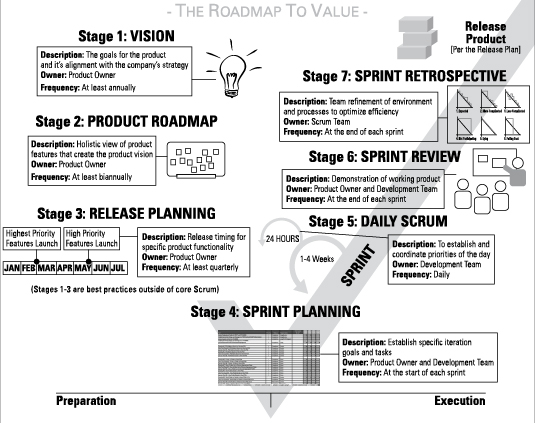
\includegraphics[width=7cm]{resources/roadmaptovalue.jpg}}
				\caption{Diagram 1: The Agile Roadmap to Value \cite{agileRoadmapToValue}}
		\end{figure}
		
		Diagram 1 shows The Roadmap to Value is a high level view of an agile project. We would use this roadmap following the term-time , which is from the first until last report and the prototype itself.
		
		In the first report, we have covered Stage 1, Stage 2 and Stage 3. The first stage we have identified the Product Vision that is briefly planned in the first section of report, which is System Requirements and Acceptance Criteria. In term of the frequency, we can change our planned task and deliverables whenever we need to. For second stage, since we have the existing codebase, even though it is not working right now, we already have the holistic view. Hence, we would improve the interface as we are working on the prototype. Next, in third stage, Table 1 below has described our Release Planning throughout the coursework timeline as a rough guide. 
		
		Apart from that, from Stage 4 until Stage 7 and the Product Release, we will explain in much more detail in accordance to our deliverables plan in Table \ref{table:agiledeliverablesplan}.
		\newpage
		\setlength{\aboverulesep}{0pt}
		\setlength{\belowrulesep}{0pt}
		{\small
		\begin{longtable}{{|p{1.7cm}|p{16cm}|p{1.7cm}|}}
			\caption{Agile deliverables plan}
			\label{table:agiledeliverablesplan}\\	
			\toprule
			No. & Task & 1 \\
			\midrule
			\endfirsthead
			\multicolumn{3}{c}%
			{\tablename\ \thetable\ -- \textit{Continued from previous page}} \\
			\midrule
			No. & Task & 1 \\
			\midrule
			\endhead
			\hline \multicolumn{3}{r}{\textit{Continued on next page}} \\
			\endfoot
			\midrule
			\endlastfoot
			
			1 & Identify system requirements: functional and non-functional system requirements & 1 \\
			\midrule
			
			2 & Identify acceptance criteria: testable acceptance criteria associated with functional and non-functional requirements & 1 \\
			\midrule
			
			3 & Discussion of legal, social, ethical and professional issue & 1 \\
			\midrule
			
			4 & Do clear work plan, discuss a suitable software development process and state focus on next phase of project & 1 \\
			\midrule
			
			5 & Study existing code & 1 \\
			\midrule
			
			6 & Modify user interface (use navigation) & 2 \\
			\midrule
			
			7 & Design database and implication (including backup scheme) & 2 \\
			\midrule
			
			8 & Forms * & 2 \\
			\midrule
			
			9 & Provide exception handling & 2 \\
			\midrule
			
			10 & Provide error checking of end-user-input & 2 \\
			\midrule
			
			11 & Fix bugs on current system & 2 \\
			\midrule
			
			12 & Have maintainable code & 2 \& 3 \\
			\midrule
			
			13 & Admin and Developer documentation & 2 \& 3 \\
			\midrule
			
			14 & Testing framework  & 2 \& 3 \\
			\midrule
			
			15 & Allow logging of student answers to be compared later on & 2 \& 3 \\
			\midrule
			
			16 & Use the Python PEP8 coding convention & 2 \& 3 \\
			\midrule
			
			17 & Authors page (camel class \& how-to) & 3 \\
			\midrule
			
			18 & Break down teachers page & 3 \\
			\midrule
			
			19 & Add methods of checking and comparing student answers from questions & 3 \\
			\midrule
			
			20 & Add deadlines to student’s homework question  & 3 \\
			\midrule
			
			21 & Provide functionality to only see modules a student enrolled for & 3 \\
			\midrule
			
			22 & Ease of use & 3 \\
			\midrule
			
			23 & System should have security permissions to prevent unauthorised access to lecturer areas. & 3 \\
			\midrule
			%\caption{Agile Deliverable Plan}
		
			\bottomrule

		\end{longtable} }
		
		\textbf{Key:} *  -  high priority
		1st report: 27/11/15 – Initial Group \& Individual Report
		2nd report: 12/11/16 – Interim Group \& Individual Report
		3rd report: 29/11/16 – Final Group \& Individual Report \& Presentation
		
		The plan of deliverables table shows our aim to complete those tasks by respective reports. Since we are doing the task in pairs or individually, we may get started on high priority tasks and the others in parallel. At the end of the second deliverable, we expect to debug any errors which it initially had, and we will ensure testing of the prototype and ensure it has maintainable code following the standard. Apart from that, the tasks that we aimed to complete on the second and third report, it is more needed to ensure the maintainability to continue to the third report. For the third report, we aimed to complete all the tasks and expect the system working for all stakeholders; lecturers, authors, students and future developers. 
	
	
    \addcontentsline{toc}{subsection}{Extreme Programming}
	\subsection*{Extreme Programming}
		Extreme Programming is also featured as a part of the Agile Software Development approach \cite{agileModeling}. Extreme Programming (XP) is also a practice related with software development. I think it is suitable with the nature of our project because Extreme Programming stresses on customer satisfaction \cite{agileXPFlowchart}. Since our project is working closely with our client, our main aim is to have accomplished the requirements that we have agreed on.  It places a strong emphasis on technical practices in addition to the more common teamwork and structural practices \cite{agileArtOfDevelopment}.
			
		Apart from that, Extreme Programming emphasizes on teamwork as customers and developers are all in a collaborative team (Extreme Programming, n.d.) \cite{agileXPFlowchart}. It is meant to be implemented in a simple yet effective environment allowing teams to become highly productive. We as a team will also be self-organized to solve problems as efficiently as we can, such as trying to  work on priority tasks based on our capabilities.
		
		Starting on second deliverables and continuing into the third report, we aim to get feedback by testing the code on weekly basis. Each requirement that we succeed to implement will deepen unique contributions by each and every team member. 
		
		This diagram below shows overview of how XP works.  
		
		\begin{figure}[!htbp]
			\centerline{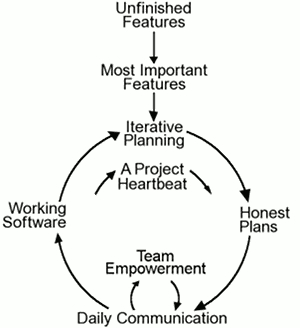
\includegraphics[width=5cm]{resources/agileflowchart.jpg}}
			\caption{Diagram 2: XP Flow chart \cite{agileXPFlowchart}}
		\end{figure}
		
		The flow of XP would compliment the situation we had, which is the existing code is an unfinished feature, then we need to identify any requirements that need to be prioritised. As time passes by, we will fulfil more requirements to enhance and improve the CAMEL system until it can be used for end users; students and lecturers.
\newpage	
    \addcontentsline{toc}{subsection}{First Group Report Gantt Chart}
	\subsection*{First Group Report Gantt Chart}
		In order to keep track of our activities and tasks on a weekly basis, a Gantt chart is used. On the left side of the Gantt chart is a list of tasks with respective starting and finishing date, duration and team members in charged. Each task is represented by a bar, which the date and length of the bar reflects the start date, duration and end date of the task. The Gantt chart for this first report has been attached in the appendices. See \ref{app:gantt}  
	
    \addcontentsline{toc}{subsection}{Conclusion}
	\subsection*{Conclusion}
		The software development method we are going to use for working on the CAMEL system is Agile Software Development, and we will specifically be using the XP approach as it compliments the nature of our project. We will try to follow the deliverables as planned so that our client’s requirements are fulfilled. Last but not least, we aimed for a working end-system and maintainability for future development.

	


	\section{Final Conclusion}
Because we have a large range of requirements to add to the existing codebase, we have decided the priorities of each of these requirements and have made a plan of when we will be able to implement them. We have also created a risk map of carrying out these requirements efficiently, and be prepared for any effects of these risks. 
We have chosen agile development as it is suited to our project and have created a gantt chart to map which team member will be able to do which requirement following the agile development plans. 
To ensure we follow legal, ethical, and social guidelines we have outlined them so that our end product will be of a high quality which breaks no laws and will not offend or raise issues with the users of the system

By finishing this report it will allow us to efficiently progress with our project and make adjustments to the system to the best of our ability to give a end product of a high standard, following the guidelines our client has given us.

  

    \newpage
	\section*{Appendices}
	\addcontentsline{toc}{section}{Appendices}
	\begin{appendices}
		\addcontentsline{toc}{subsection}{Gantt Chart}
		\label{app:gantt}
		\subsection*{Gantt Chart}
		\begin{minipage}{\textwidth}
			\begin{flushright}
				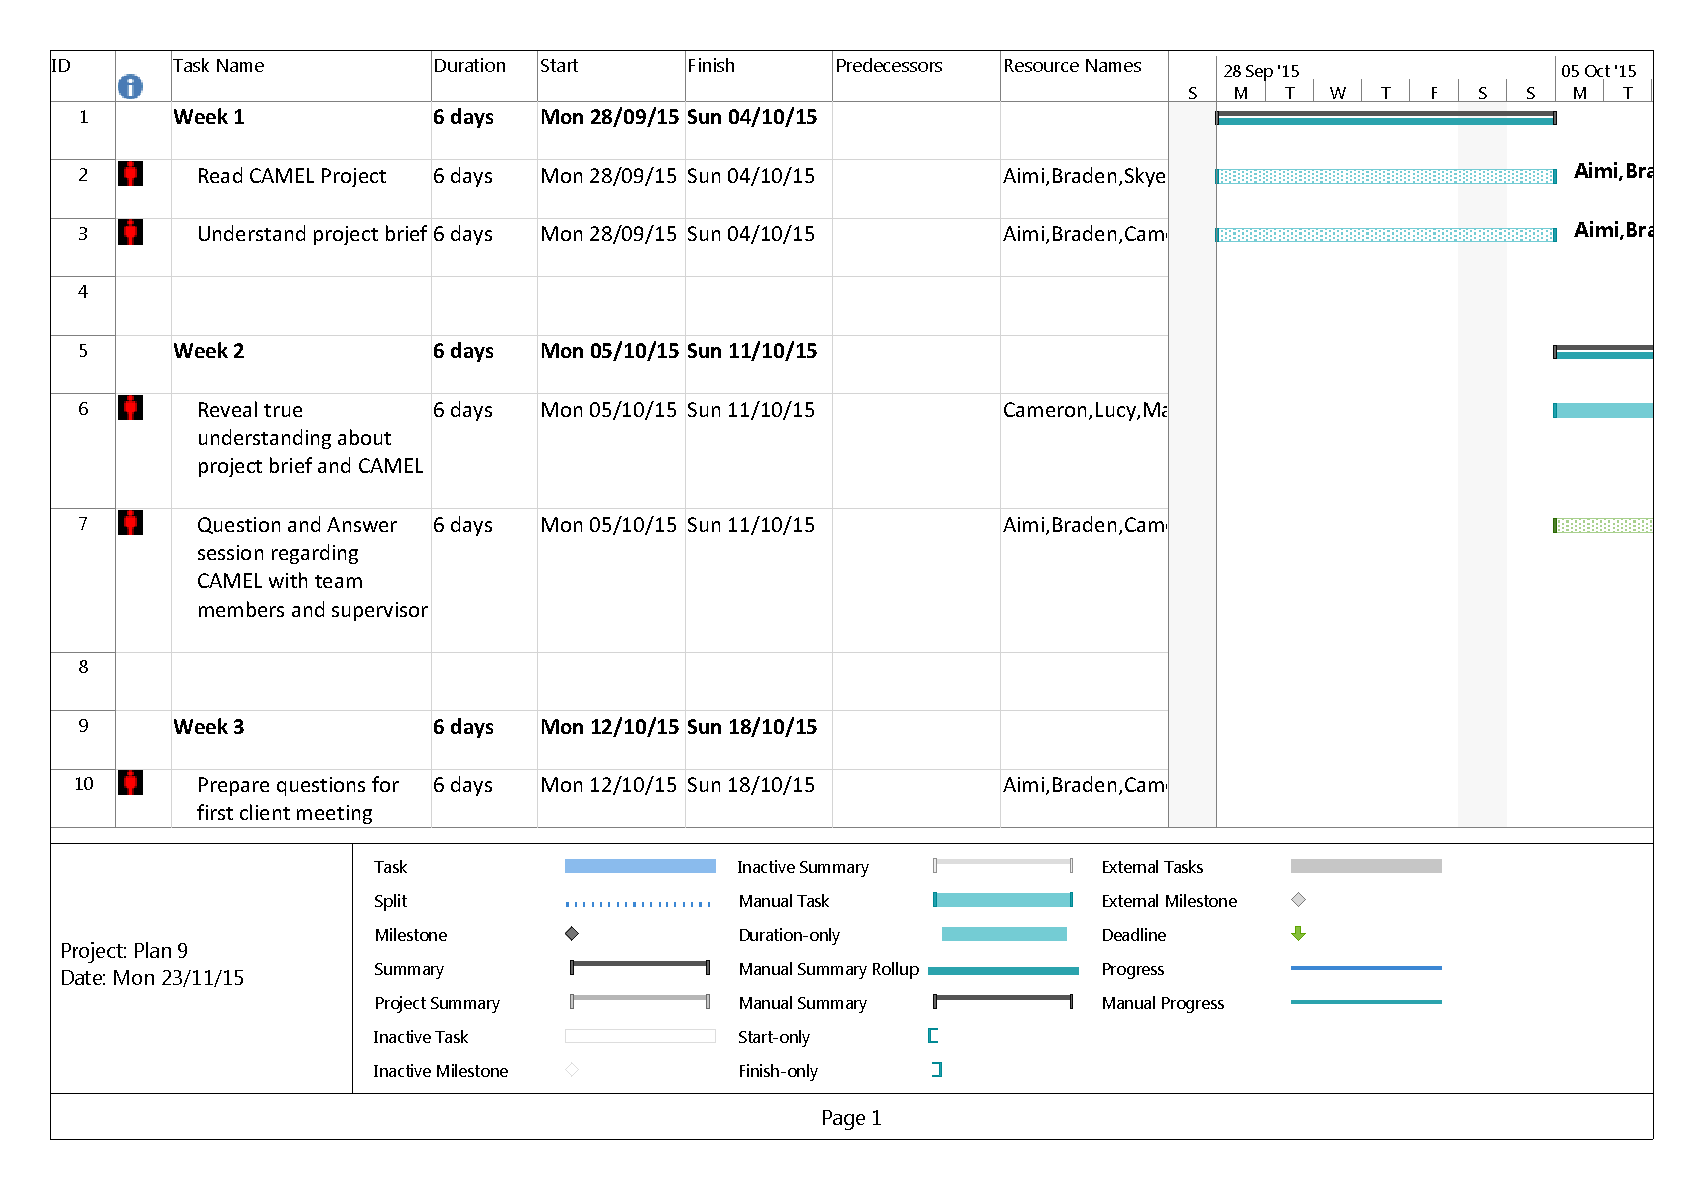
\includepdf[scale=0.75,landscape=true]{./resources/figureGanttChart.pdf}
			\end{flushright}
		\end{minipage}
	\end{appendices}
	\newpage
    \addcontentsline{toc}{section}{References}
    \printbibliography
   \end{document}
